\section{Discussion}
To understand how the structure of collaboration influences article quality, we have applied and tested the {\it bi-partite network random walker} model in the context of Wikipedia. Our results show that the model accounts well for the quality of articles  $\langle \rho_a \rangle  \approx 0.64$ and for the expertise of contributors $\langle \rho_e \rangle  \approx 0.72$, and overall exhibits a high degree of fitness. Moreover, $\rho_a$ remains stable over time, while $\rho_e$ increases, suggesting that the model reflects better editor expertise as more contributions to a broader set of articles occur, i.e., when the bi-partite network gets more densely connected. This suggests that loosely connected entities, either articles and editors, cannot be ranked accurately. From Figure \ref{fig:triangle} and from Table \ref{tab:statistics}, we see that there are always significantly more editors than articles for each category. Hence, the probability for an article to get contributions early on is higher than the probability to find editors who have contributed to a lot of articles early. 

To account for single-minded editors who have concentrated on only one or few articles, we have tested the{\it bi-partite random walker} model with a different input, namely the matrix of edit counts (instead of a binary matrix). As shown on Figure \ref{fig:binary_vs_editcount}, the model using the {\it edit counts} input matrix accounts nearly as well for article quality, while it does a much worse job ranking editor expertise compared to a {\it binary} input matrix. Counterintuitively, we observe a ``less is more" situation: the number of articles ever touched by an editor reflects better the structure of collaboration and value creation,  compared to edit counts, a much richer information input. Also, the labor-hour ground truth metric for editors is more a proxy of number of edits rather the number of articles ever touched \cite{geiger2013}. Nevertheless, the model does not perform as well with {\it edit counts} as an input. This suggests that what really counts for assessing the expertise of an editor is the number of articles touched, rather than the number of edits per article.

\begin{figure}[!t]
\centering
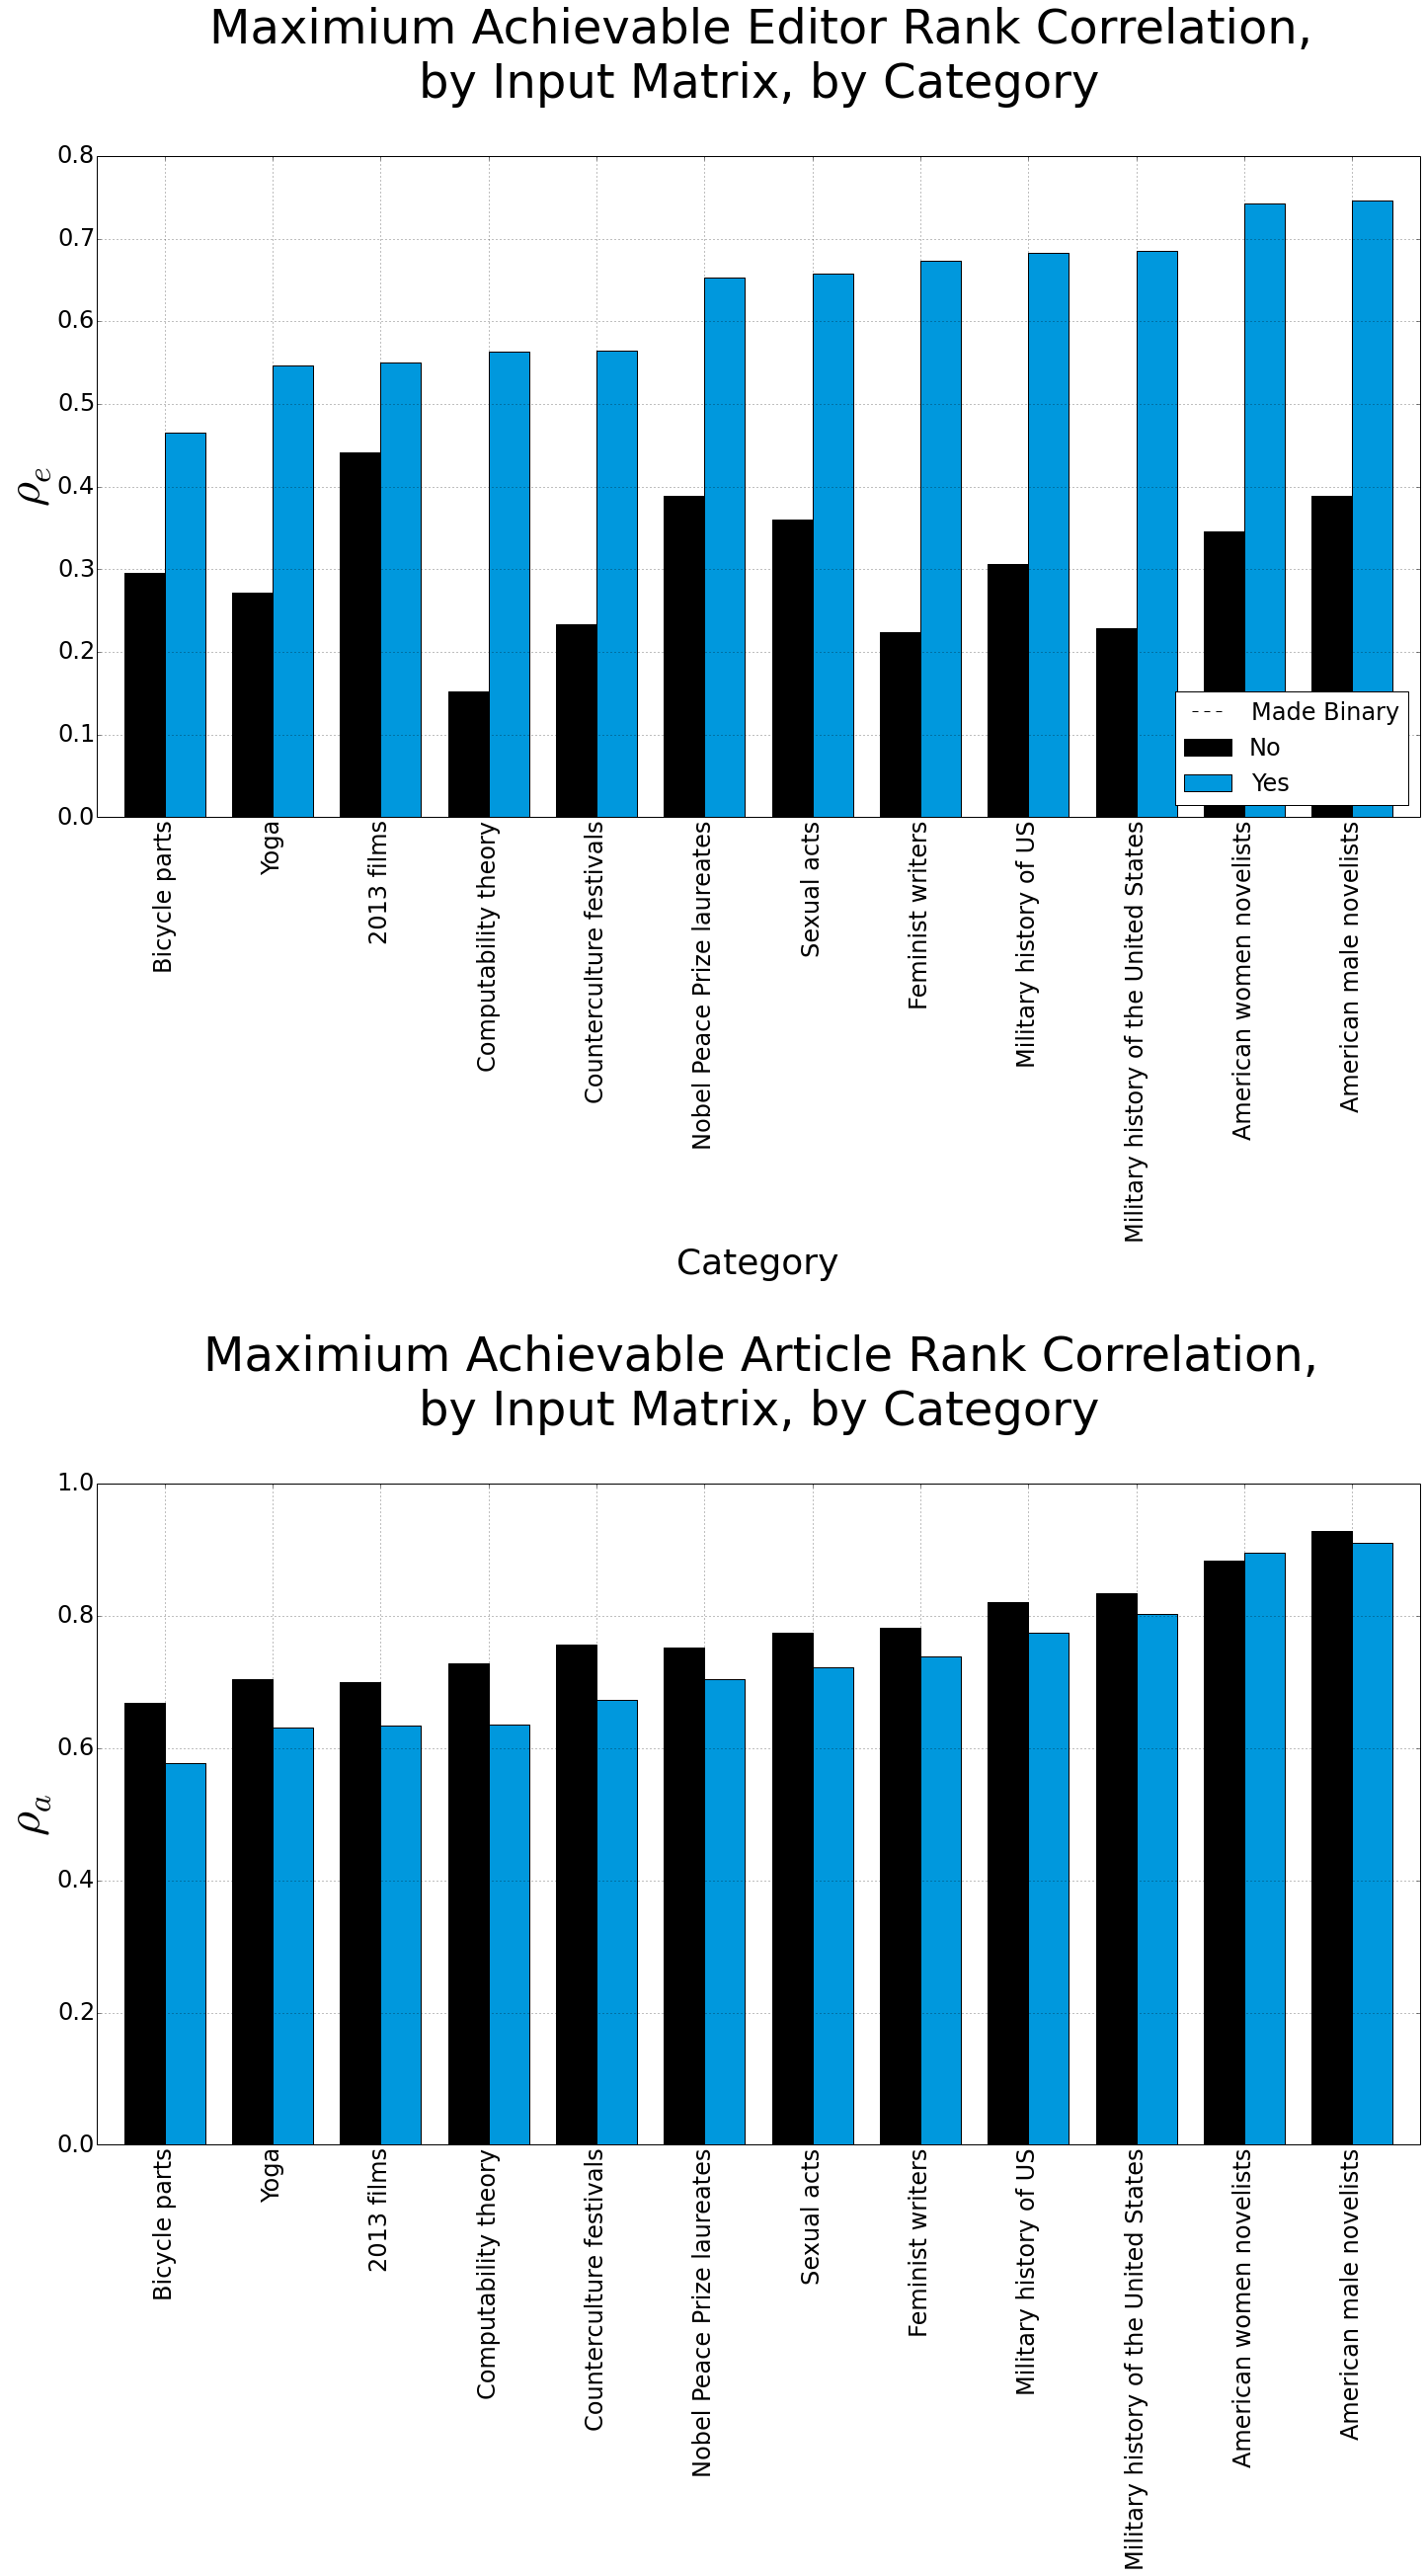
\includegraphics[width=0.9\columnwidth]{../Figures/bin_comp.png}.
\caption{Comparison between $\rho_a$ (upper panel) and $\rho_e$ (lower panel) for two input matrices: binary (black) and edit counts (blue) for each category numbered according to Table \ref{tab:maxbeta}. While taking edit counts as the input matrix only marginally increases $\rho_a$, it drastically reduces $\rho_e$.}
\label{fig:binary_vs_editcount}
\end{figure}

We now discuss how the fitted parameters $\alpha^{*}$ and $\beta^{*}$ inform on the structures of collaboration in Wikipedia categories. On the one hand, we have found $\alpha^{*} \approx 0$ for all categories, reflecting the positive influence of the number of articles edited on editor expertise. This result is compatible with previous results by Keegan et al. \cite{keegan2012}. On the other hand, $\beta^{*}$ varies across categories with values ranging from $0$ to $1.52$ at the last snapshot. $\beta$ can be considered as a measure of the collaboration structure: the smaller $\beta$, the more articles benefit from more editors. On the contrary, the larger $\beta$, the more articles benefit from less editors. If we consider for instance {\it Sexual acts}, a category that could be considered taboo or perverse with articles being the least collaboratively edited: $\beta > 1$ reflects that an editor with edits to many articles will see her ranking drop. Indeed, it should not be taken for granted that contributions are necessarily positive. Because of their socially-sensitive nature, articles about sexual acts are particularly prone to attracting vandals or edit-warring behaviors across the whole category. Therefore, editors making the most edits are not necessarily the ones improving article quality, as we would typically expect. This result is again compatible with previous research, which has shown that, in some circumstances, most active editors exhibit deleting behaviors that lower metric-based article quality ratings \cite{kane2011}. 

Conversely, the category {\it Military History of the US} is famous for its self-organized task-forces. At the latest snapshot $\beta = 0$, and is the one of only a few categories we have analyzed, which exhibits $\beta$ consistently negative over time. Accordingly, the marginal quality of articles is positively influenced by the number of editors touching the article. Unsurprisingly, {\it Military History of the US} is literally a ``WikiProject" with a hierarchy of coordinators, an active IRC channel, and a mailing list. As a result of better coordination, there is less edit-warring and more efficient contributions: editors edit articles with well-defined task at hand. 


%It requires a frictionless, collaborative environment where the more you edit, the more and more experienced you become. It's also worth noting that \cite{keegan2012}, found that ``coordination demands influence the tendency of editors with similar levels of experience to work together". \textcolor{red}{In our scenario that would mean that the coordination present attracts super-users to work in the productive environment. The category Military History is empirically a standout case of collaboration, and shows in its calibrated $\beta$ measurements. }




%This fact tells actually a lot about the model.  The actual metric for editor expertise takes only into consideration the labor hours \cite{geiger2013}, and the more time is spent editing a category, the more likely the editor will have modified a large quantity of articles. The value of $\alpha$ can therefore be explained entirely by the nature of the ground-truth metric. 

%This difference might be due to the roughness of the actual metrics for editors $\bar{w}_e$, expressed in labor-hours, compared to the quality of $\bar{w}_a$, which is an aggregate measure of five precise quality metrics. Nevertheless, the correlation of editor ranking with $\bar{w}_e$ increases: $\rho_e$ exhibits a convex increase over time, suggesting that it takes time (i.e. lots of articles edited) to capture well the expertise of editors. 

%Although it would require further testing with a broad variety of metrics, it seems that the {bi-partite network random walker} model can {\it tune} to whatever ground-truth metric used for calibration. In other words, the values of $\alpha$ and $\beta$ only reflect the structure of value creation in open collaboration, {\it given} the chosen ground-truth metrics. 


% Allowing for a moment, $\alpha = 0$ we can simplify our analytic solutions to gain a more intuitive interpretation of the calibration results.}

% %\begin{cases}
% \begin{equation}
% w^{*}_{e} \sim k_{e}^{1-\beta}\langle k_{a}^{-\alpha} \rangle_{e},\\
% w^{*}_{a} \sim k_{a}^{1-\alpha}\langle k_{e}^{-\beta} \rangle_{a}
% \end{equation}
% %\end{cases}
% 
%Then letting $\alpha = 0$, we can simplify to:
%%\begin{cases}
%\begin{equation}
% w^{*}_{e} \sim k_{e}^{1-\beta}\\[7pt]
% w^{*}_{a} \sim k_{a}
% \langle k_{e}^{-\beta} \rangle_{a}\\[7pt]
% \end{equation}
% %\end{cases} 





%\textcolor{red}{That fact that we find two very different cases of collaborativeness is important in explaining previous contention in computer support collaborative work sphere. Early on, research was release to suggest that high editor inequality among editors is related to high article quality \cite{kittur08}. The intuition is that the top superusers can be unrivaled in shaping the articles. We have certainly found this to be true in the Military History example. Yet later, it was found that editor inequality relating to article quality is unsupported, and editor inequality relating to coordination is false \cite{arazy}. In the case of chaotic categories like Sexual Acts we found this case, where the top users cannot make as much a positive impact as otherwise. These two seemingly contradictory findings can be explained through our measure of collaborativeness. Each part of wikipedia can exhibit different and measurable relationships between editor quality and article quality - that is our collaborativeness $\beta$. }

%$\mathbf{M}$ : most basic measure of collaboration, which represents the bi-partite network contributions to articles by editors: Here, we consider the simplest information available on collaboration: has an editor modified an article at any point in time or not ?


%Analyzing the Creative Editing Behavior of Wikipedia Editors: Through Dynamic Social Network Analysis \footnote{This paper analyzes editing patterns of Wikipedia contributors using dynamic social network analysis. We have developed a tool that converts the edit flow among contributors into a temporal social network. We are using this approach to identify the most creative Wikipedia editors among the few thousand contributors who make most of the edits amid the millions of active Wikipedia editors. In particular, we identify the key category of �coolfarmers�, the prolific authors starting and building new articles of high quality. Towards this goal we analyzed the 2580 featured articles of the English Wikipedia where we found two main article types: (1) articles of narrow focus created by a few subject matter experts, and (2) articles about a broad topic created by thousands of interested incidental editors. We then investigated the authoring process of articles about a current and controversial event. There we found two types of editors with different editing patterns: the mediators, trying to reconcile the different viewpoints of editors, and the zealots, who are adding fuel to heated discussions on controversial topics. As a second category of editors we look at the �egoboosters�, people who use Wikipedia mostly to showcase themselves. Understanding these different patterns of behavior gives important insights about the cultural norms of online creators. In addition, identifying and policing egoboosters has the potential to increase the quality of Wikipedia. People best suited to enforce culture-compliant behavior of egoboosters through exemplary behavior and active intervention are the highly regarded coolfarmers introduced above. }\cite{iba2010}


%{\bf Network Analysis of Collaboration Structure in Wikipedia} \footnote{In this paper we give models and algorithms to describe and analyze the collaboration among authors of Wikipedia from a network analytical perspective. The edit network encodes who interacts how with whom when editing an article; it significantly extends previous network models that code author communities in Wikipedia. Several characteristics summarizing some aspects of the organization process and allowing the analyst to identify certain types of authors can be obtained from the edit network. Moreover, we propose several indicators characterizing the global network structure and methods to visualize edit networks. It is shown that the structural network indicators are correlated with quality labels of the associated Wikipedia articles.} \cite{brandes2009}


%The problem of ranking entities and their respective production is relevant to the flourishing production of knowledge on the Web, and is directly related to two outstanding problems, which have been previously debated. First, how do we gauge the quality (resp. reliability) of blog posts, book reviews (e.g. on Amazon), or restaurant reviews (e.g. on Yelp) ?  Second,  how to grant editing and administrative privileges on community networks (e.g. Slashdot) and on online collaborative platforms (e.g. Wikipedia) \cite{halfaker2013}. 
